\section{Evaluation}
\label{sec:evaluation}
In this section we evaluate the chatbot tool we created for this project. We
use a set of questions to evaluate the performance of the chatbot. For question
we provide the best response from our chatbot along with a piece of context we
have from the documentation of the Fogify tool. This way we compare the results
of the chatbot in comparison with the context of the documentation. Below we
provide the set of questions we asked our chatbot, along with some context from
the documentation page of Fogify.

\subsubsection*{Questions used in the evaluation stage}
\begin{enumerate}
    \item What is an action and how can i add an action using python code?
          \begin{itemize}
              \item An "Action" is a process that changes the properties of a
                    running Fog Topology. Due to extensibility, we introduce a
                    general
                    "action"
                    method in which users can utilize. As we described earlier,
                    the
                    method needs
                    the "action\_type" parameter, which currently could be one
                    of the
                    following:
                    "HORIZONTAL\_SCALING",
                    "VERTICAL\_SCALING", "NETWORK", "STRESS", "COMMAND", and
                    the action's "parameters". The "parameters" is a dictionary
                    with
                    all
                    necessary
                    variables of an action and the emulated instance "label"
                    that the
                    action will
                    be apply to.
                    "fogify.action(action\_type, **parameters)"
          \end{itemize}

          \begin{figure}[h!]
              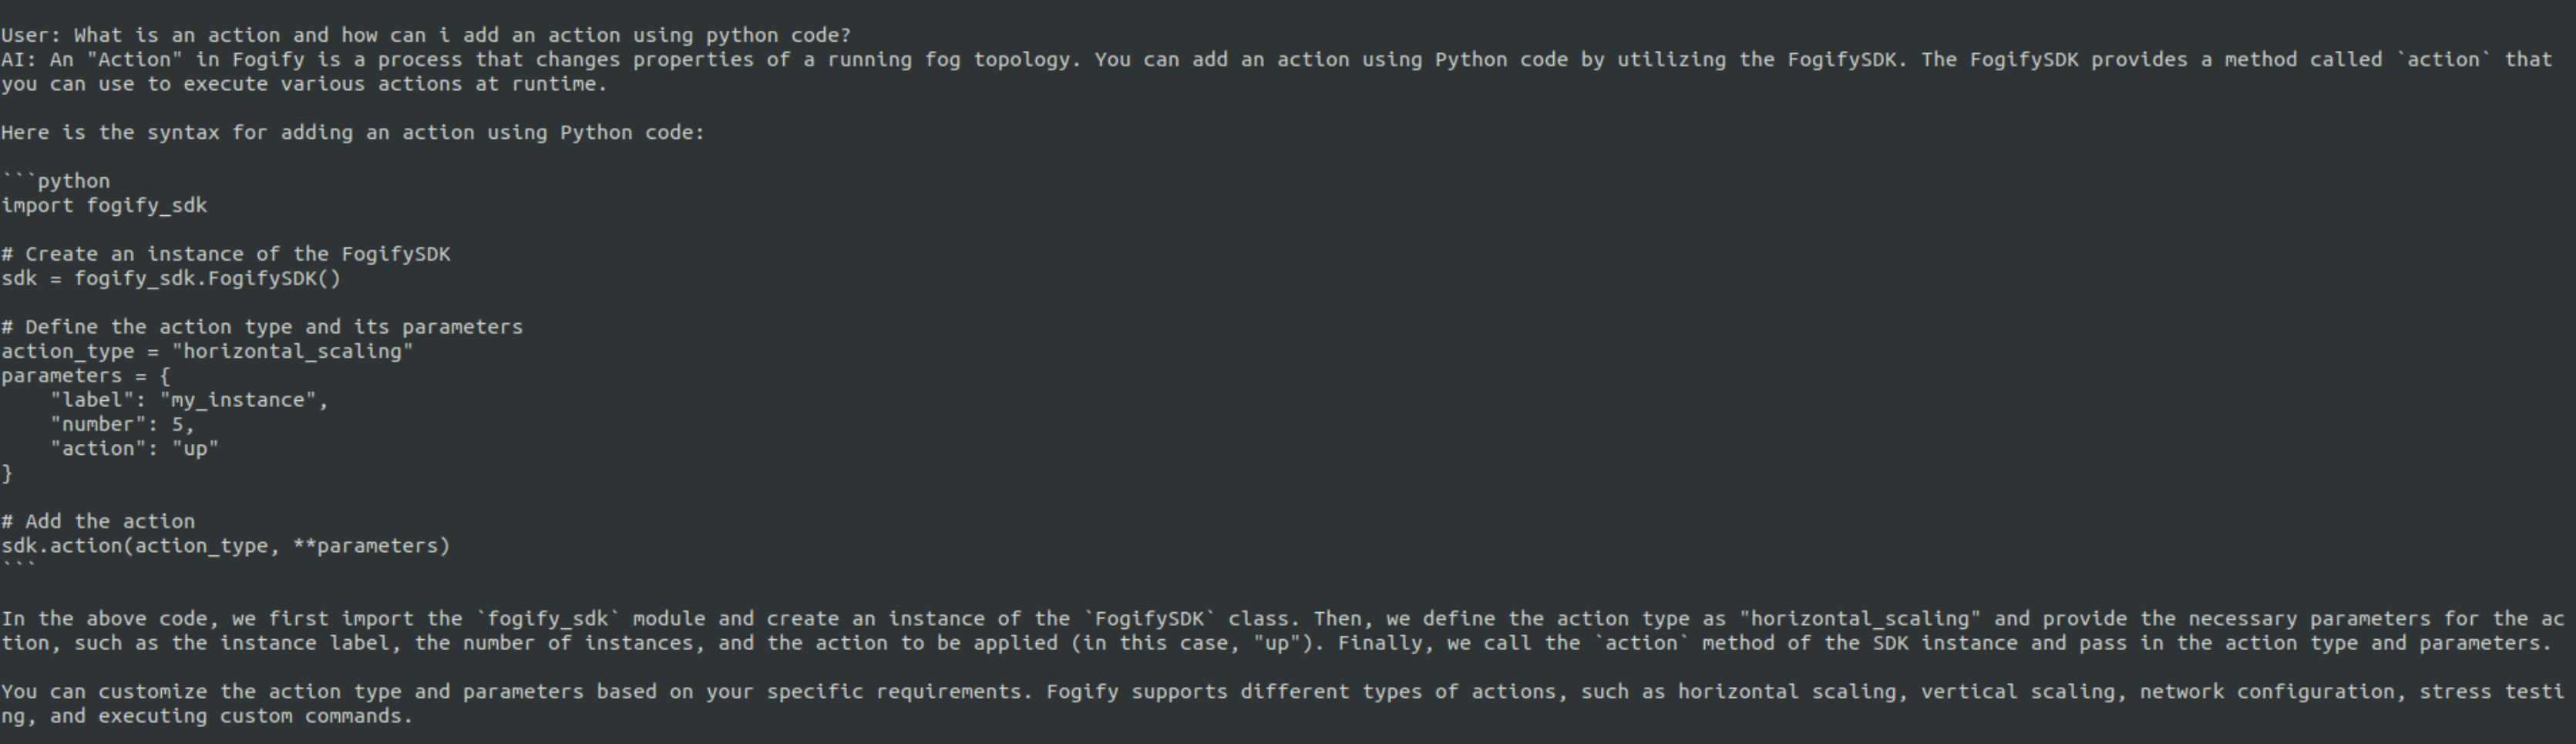
\includegraphics[width=8cm,height=4cm]{figures/q1.png}
              \caption[Methodology pipline]{Answer for question 1}
              \label{img:q1}
          \end{figure}
    \item What are some parameters that we specify in the Fogify emulator for
          network connectivity? Can you give me an example of yaml
          configuration?
          \begin{figure}[h!]
              \includegraphics[width=8cm,height=4cm]{figures/q2\_cor.png}
              \caption[Methodology pipline]{Correct Answer for question 2}
              \label{img:q2_cor}
          \end{figure}

          \begin{figure}[h!]
              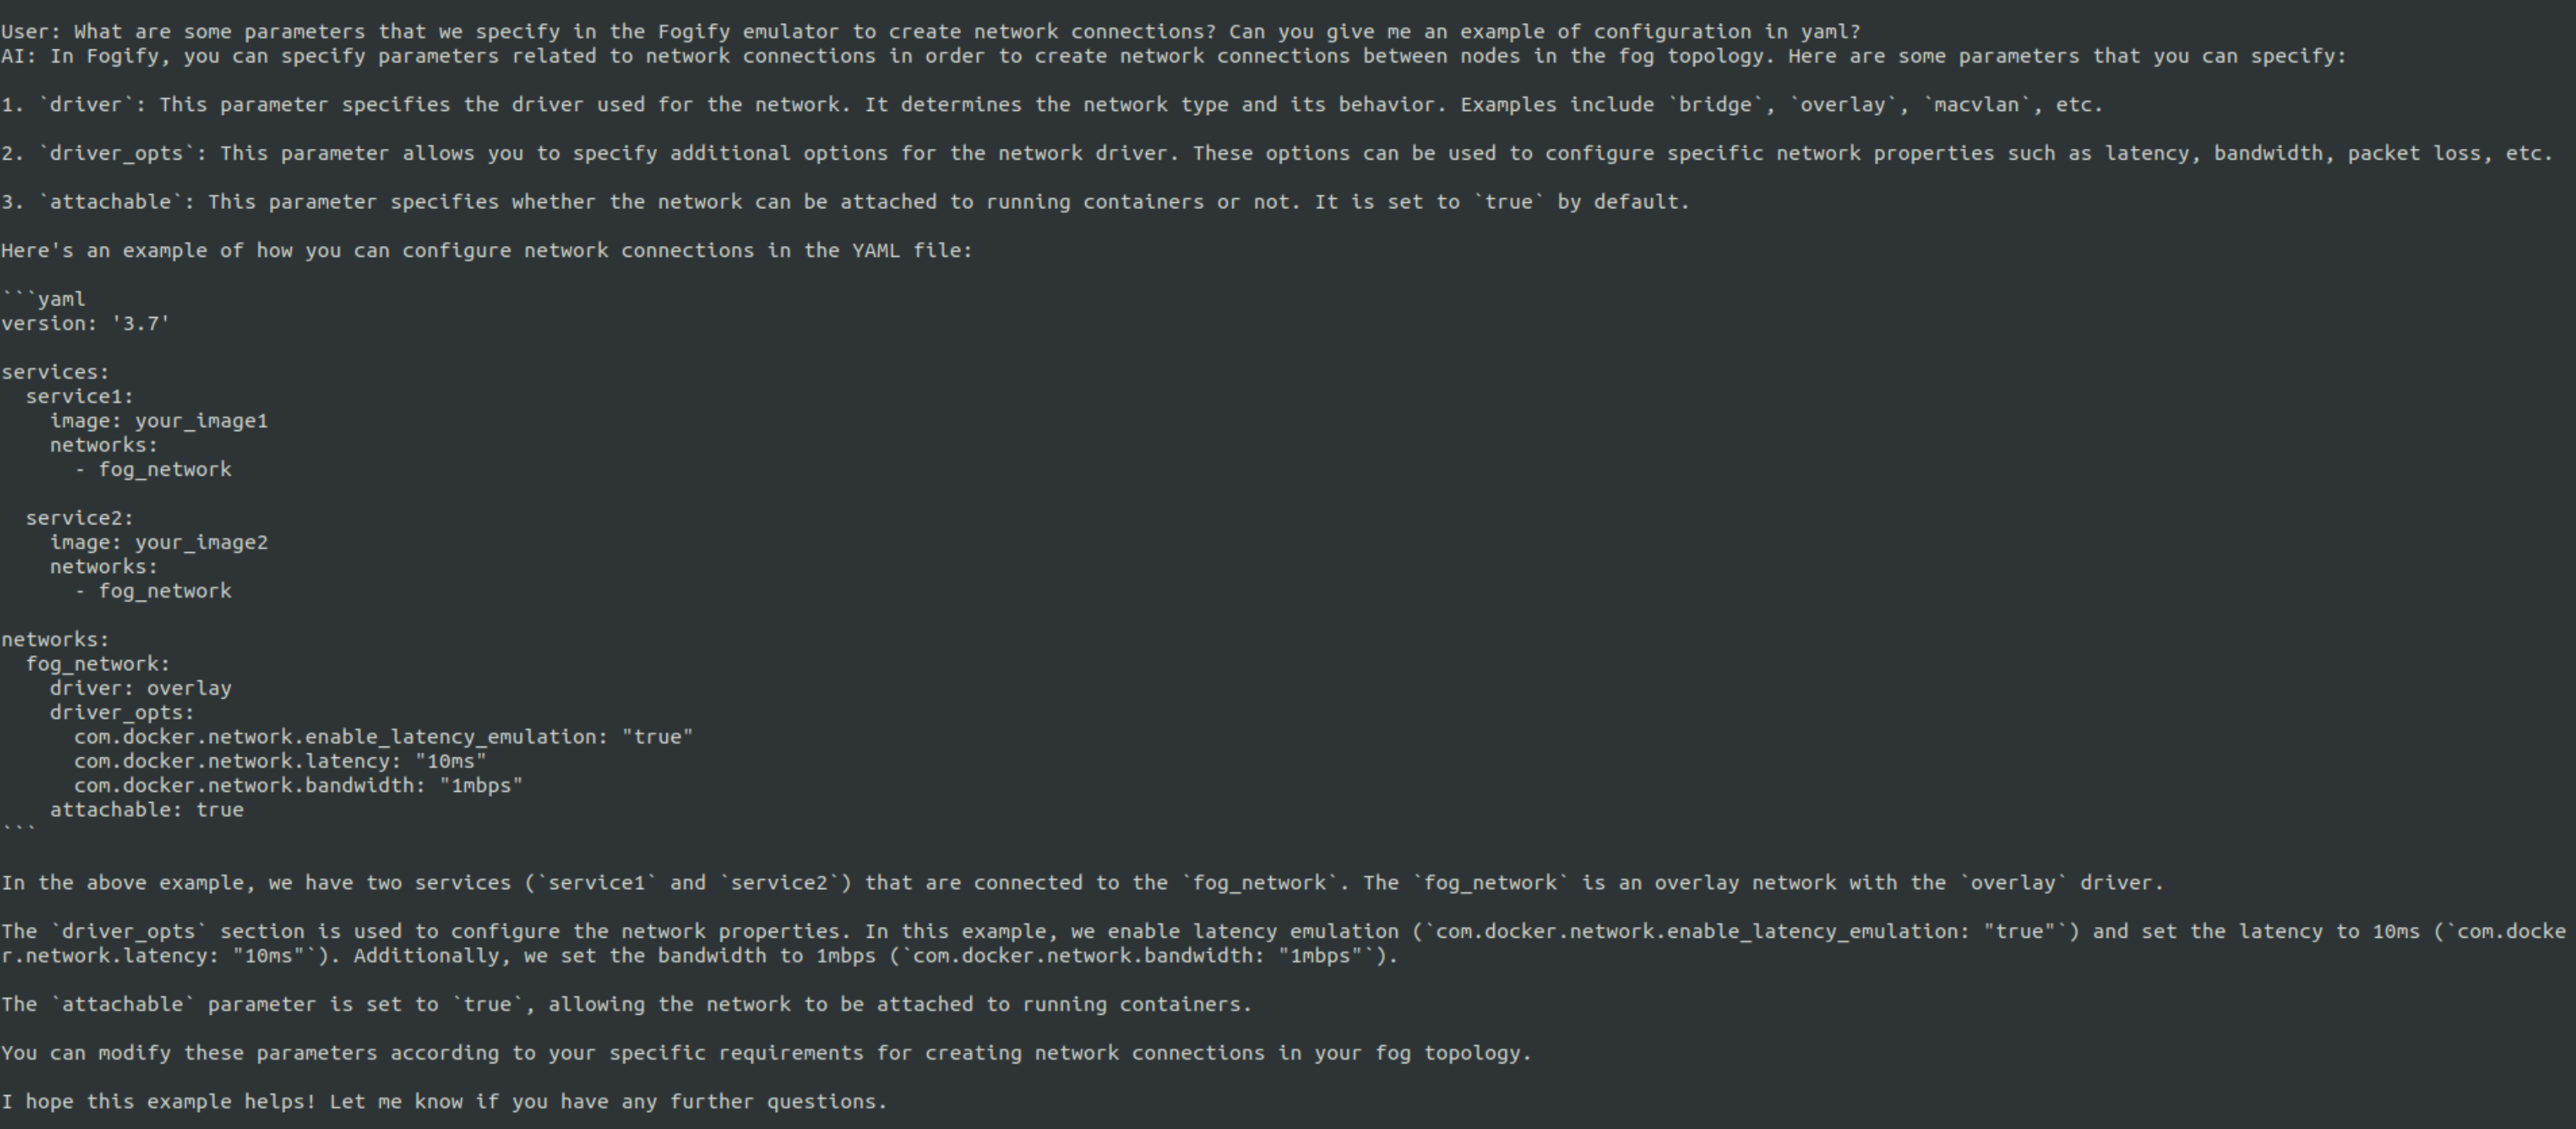
\includegraphics[width=8cm,height=4cm]{figures/q2.png}
              \caption[Methodology pipline]{Answer for question 2}
              \label{img:q2}
          \end{figure}
    \item What are blueprints and what are their different variables? Can you
          also give me an example?
          \begin{itemize}
              \item
          \end{itemize}
          \begin{figure}[h!]
              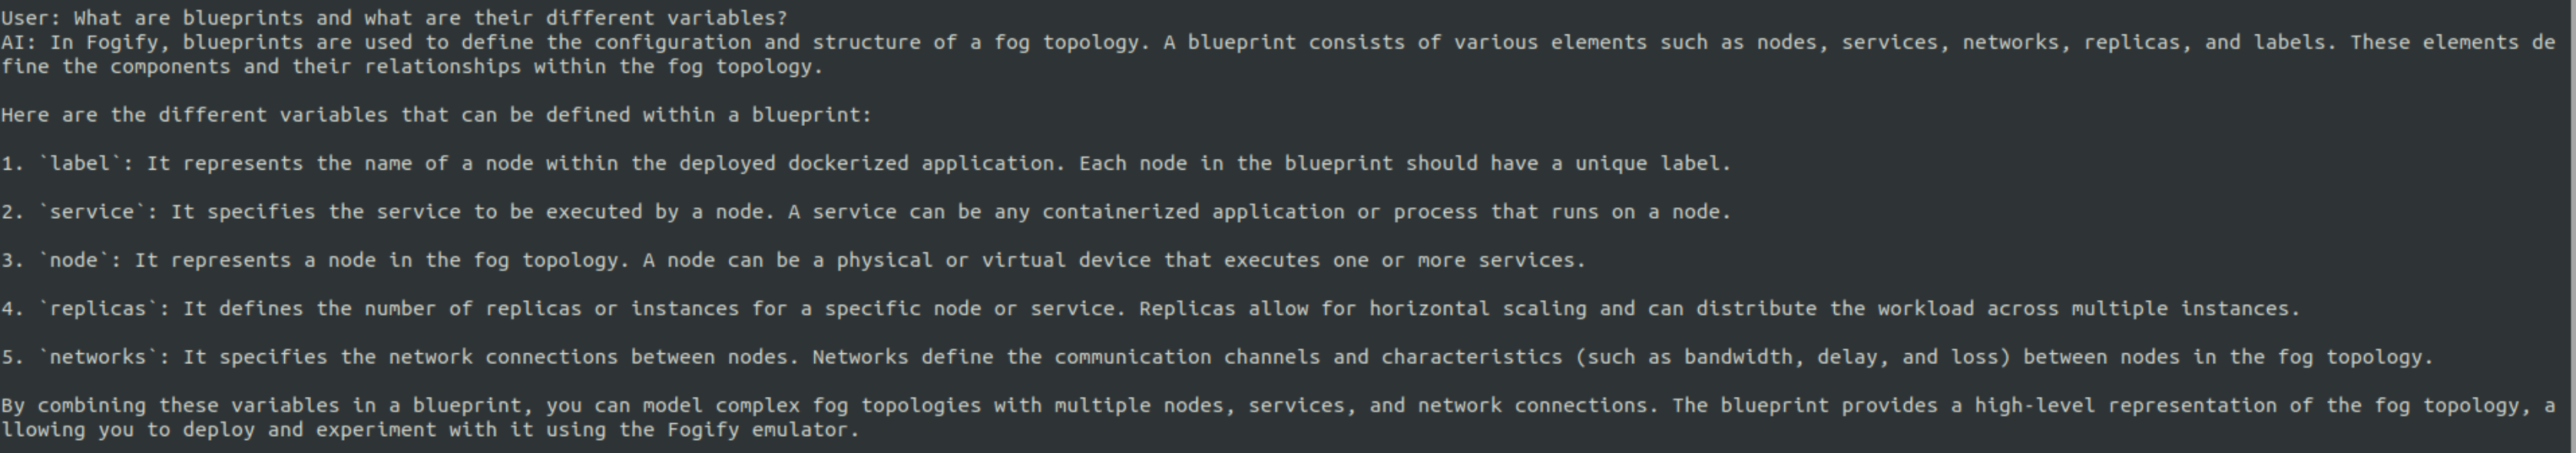
\includegraphics[width=8cm,height=4cm]{figures/q3.png}
              \caption[Methodology pipline]{Answer for question 3}
              \label{img:q3}
          \end{figure}
    \item How does Fofigy compose the network latency can you give me an
          example of configuration with the different variables in that yaml?
          \begin{itemize}
              \item
          \end{itemize}
          \begin{figure}[h!]
              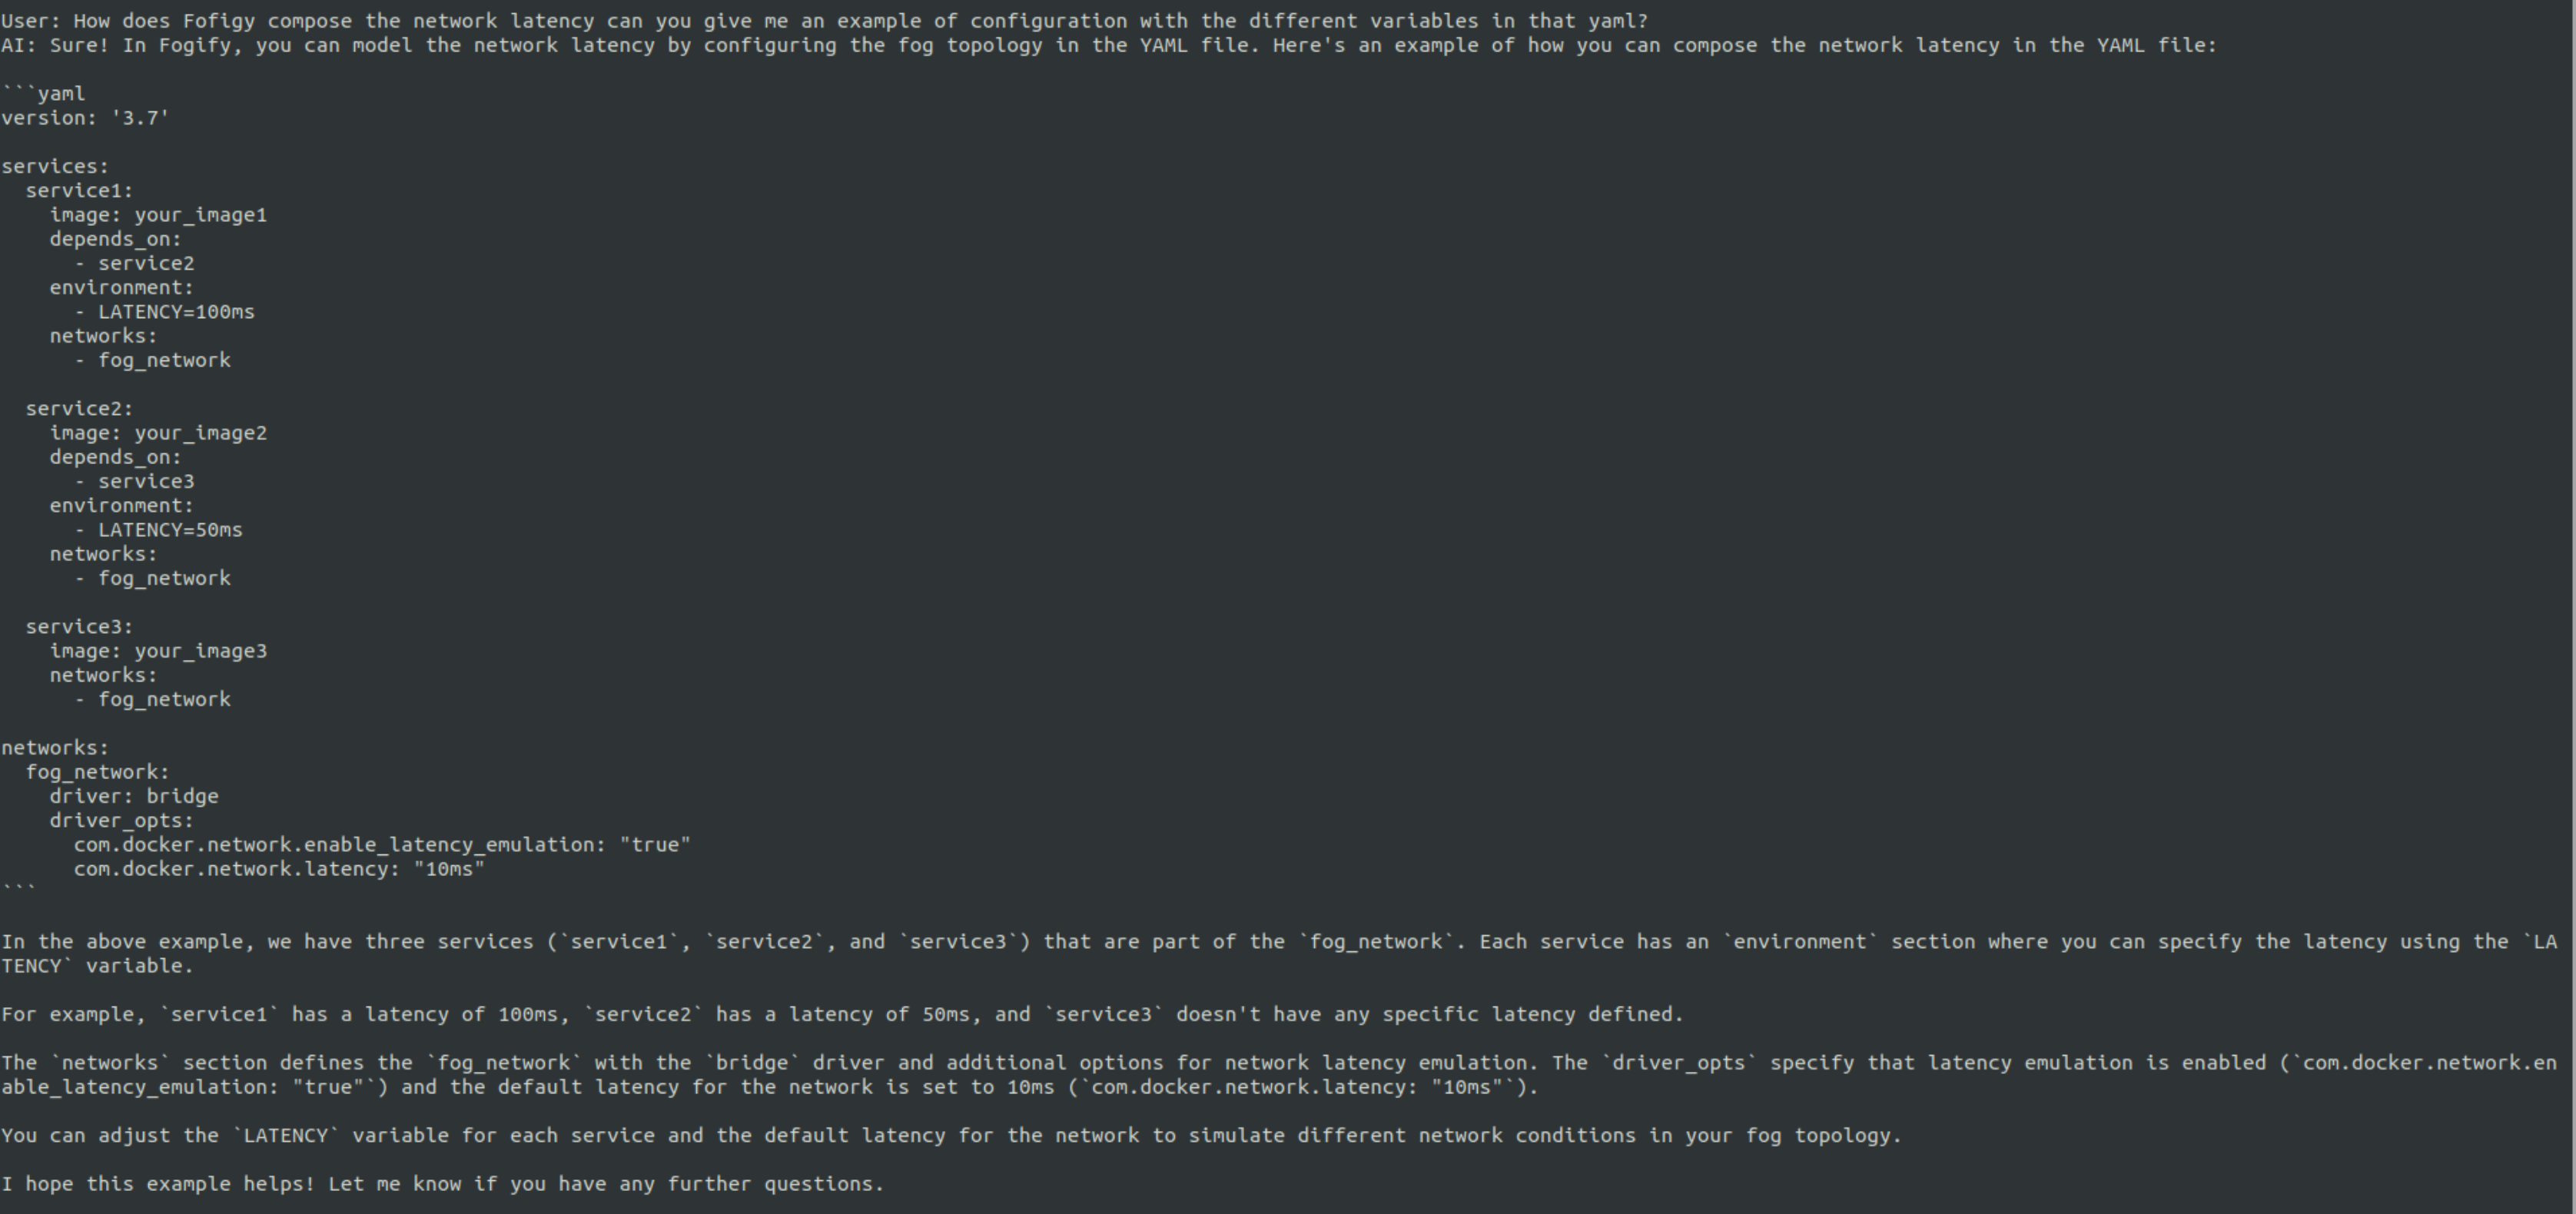
\includegraphics[width=8cm,height=4cm]{figures/q4.png}
              \caption[Methodology pipline]{Answer for question 4}
              \label{img:q4}
          \end{figure}
    \item Explain the different parameters of the blueprint.
          \begin{itemize}
              \item
          \end{itemize}
          \begin{figure}[h!]
              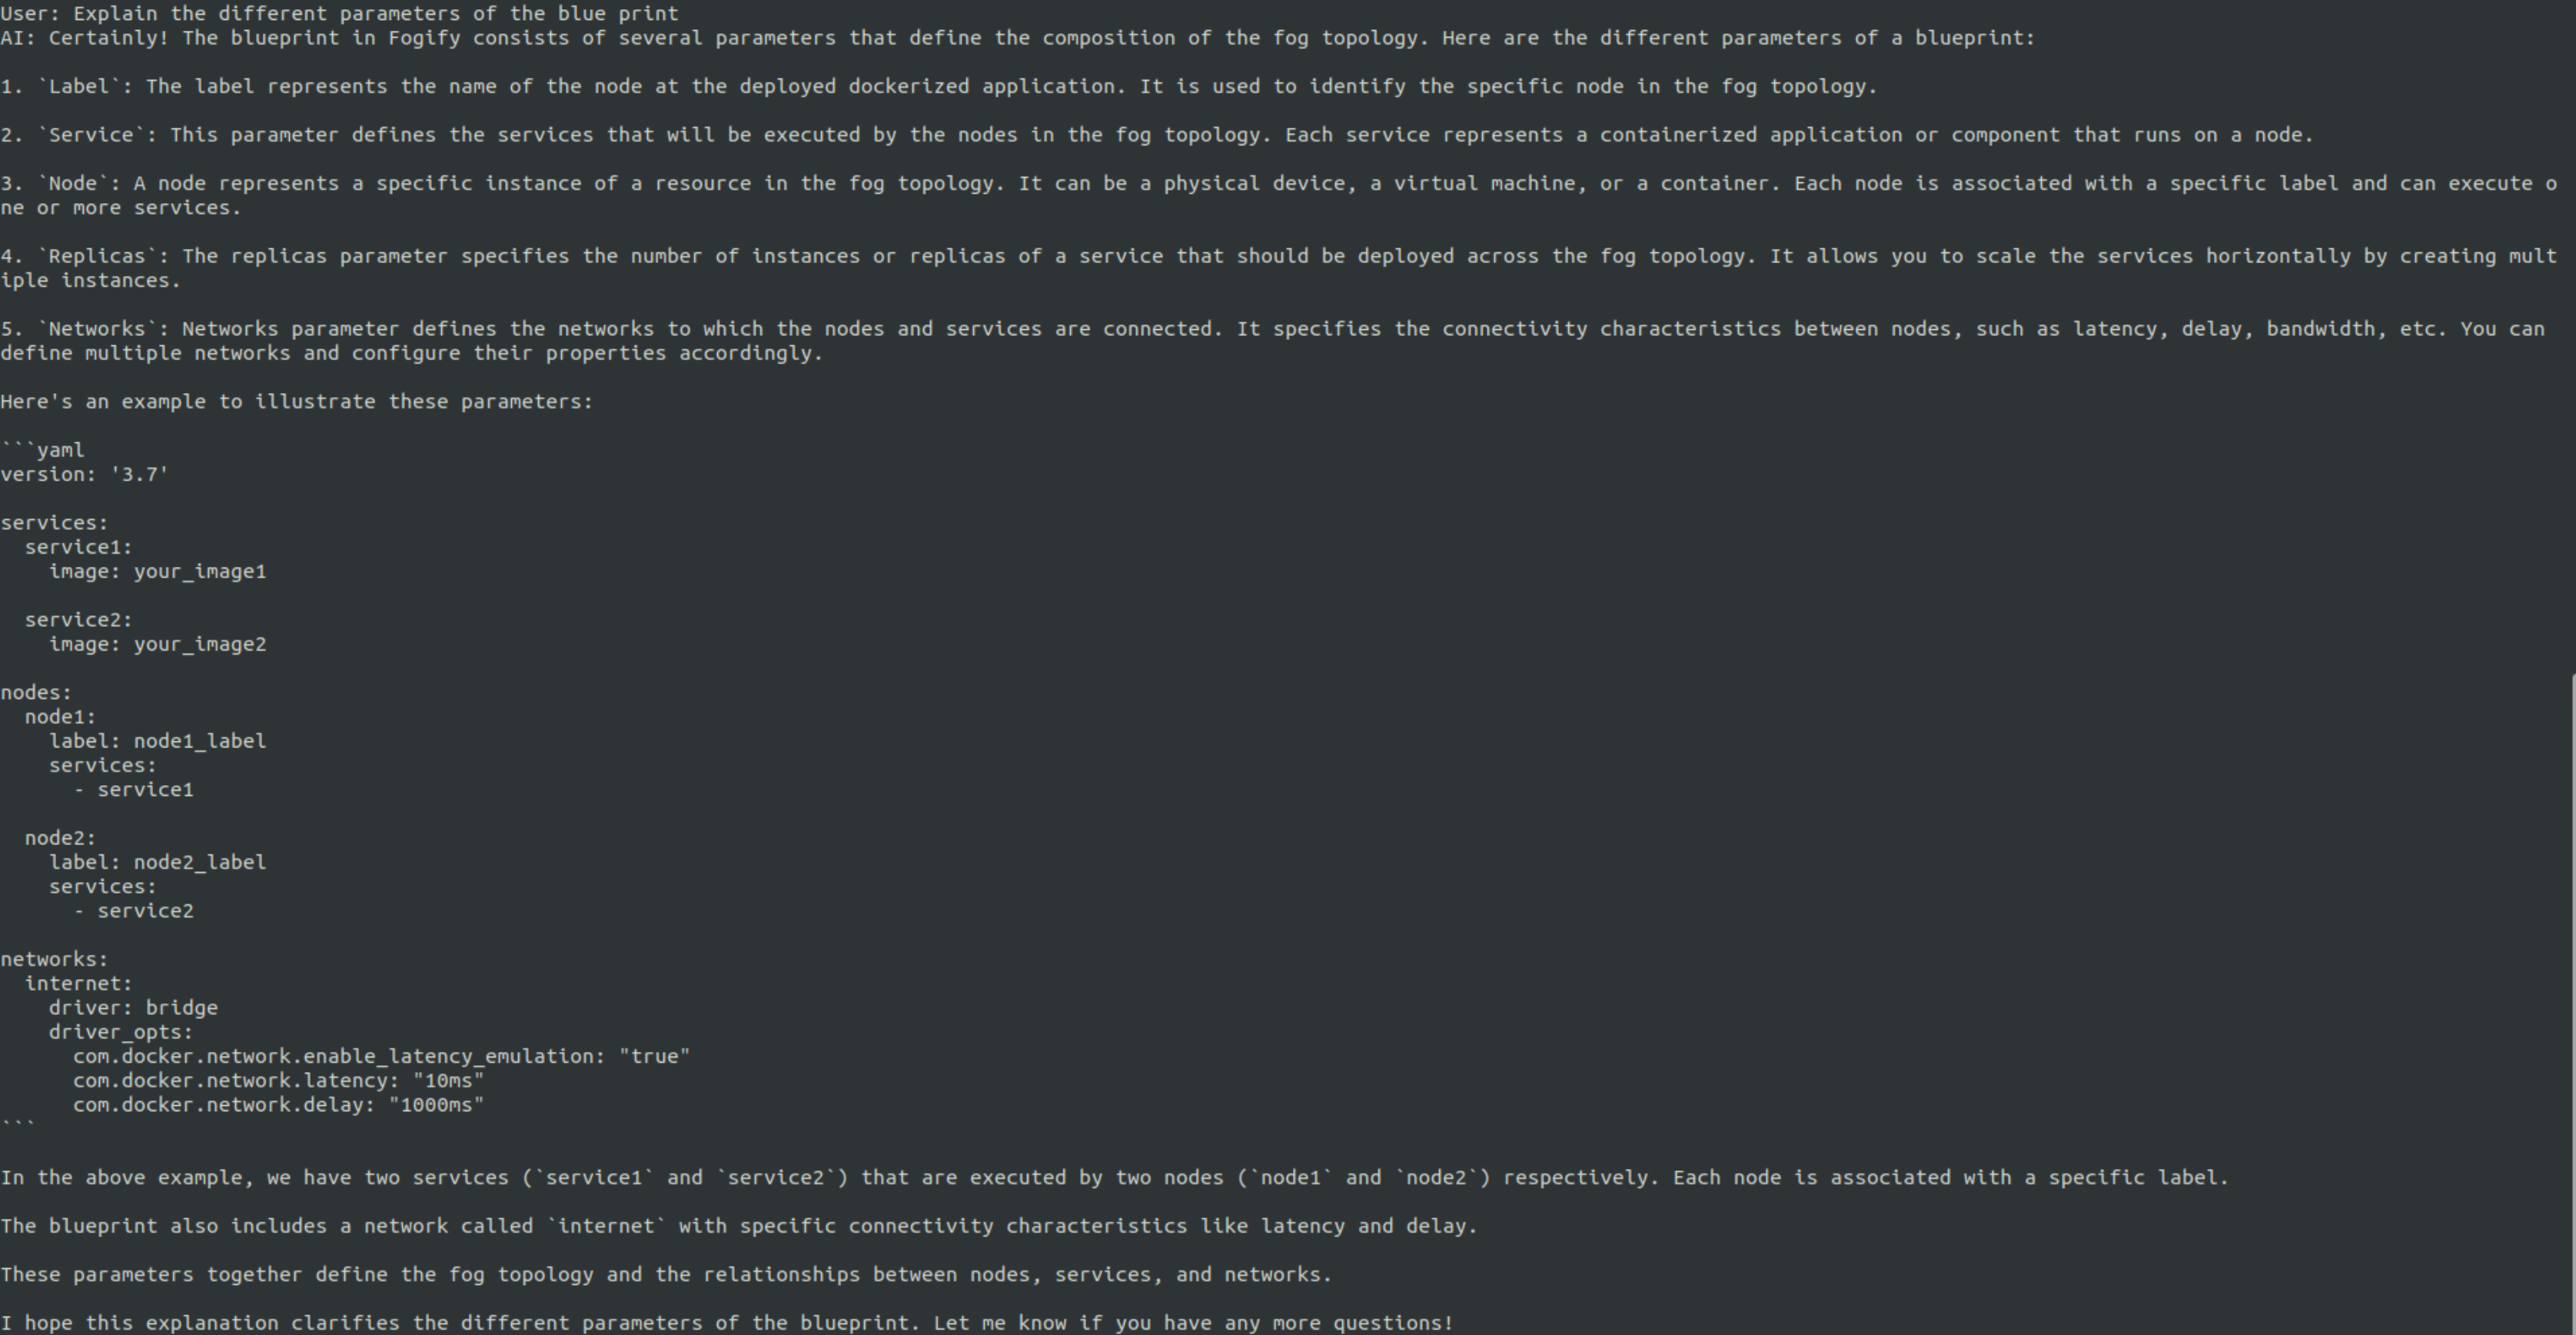
\includegraphics[width=8cm,height=4cm]{figures/q5.png}
              \caption[Methodology pipline]{Answer for question 5}
              \label{img:q5}
          \end{figure}
    \item What are the performance metrics captured by Fogify. Can you give me
          the metric and a small description for it?
          \begin{itemize}
              \item
          \end{itemize}
          \begin{figure}[h!]
              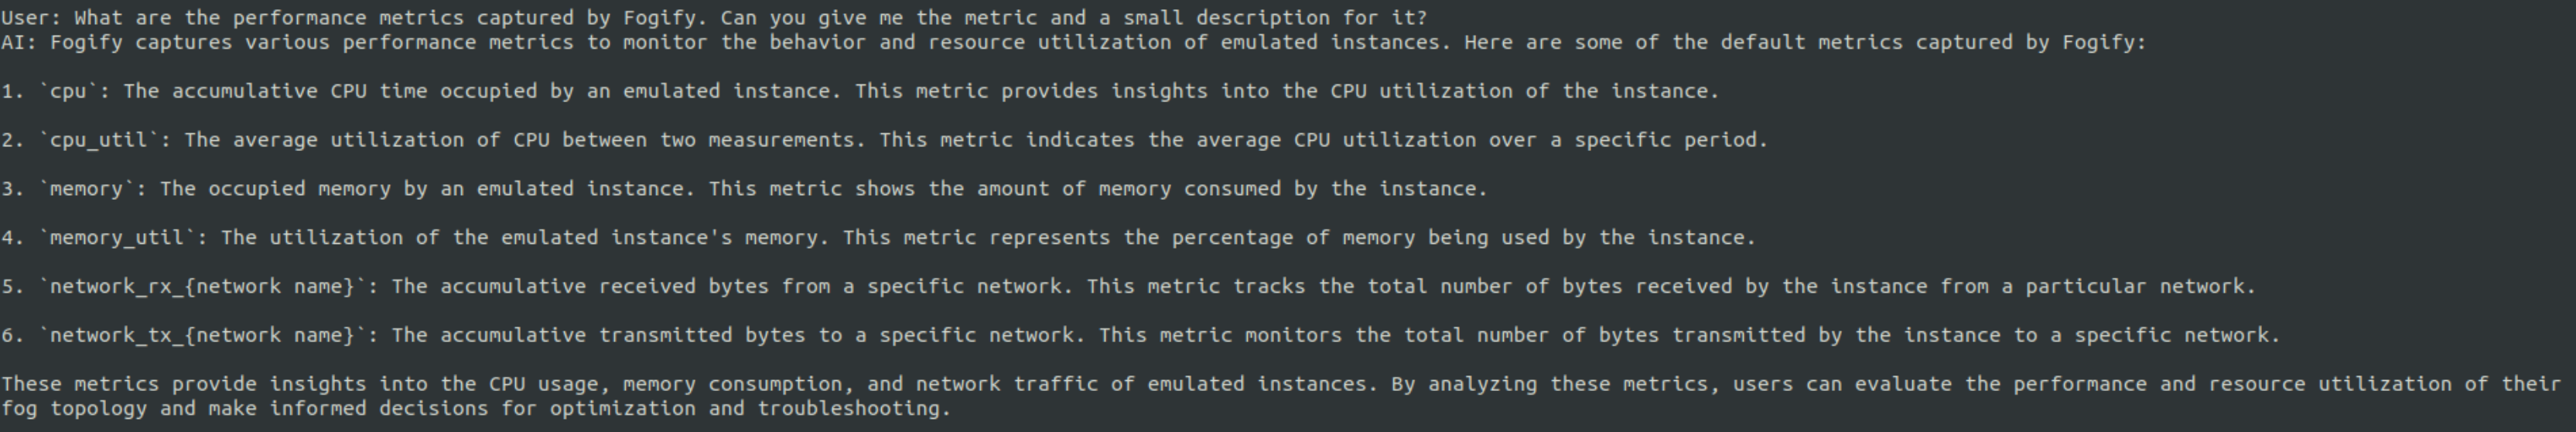
\includegraphics[width=8cm,height=4cm]{figures/q6.png}
              \caption[Methodology pipline]{Answer for question 6}
              \label{img:q6}
          \end{figure}
    \item Can a user add its own metrics to fogify? How can a user do that can
          you give me an example?
          \begin{itemize}
              \item
          \end{itemize}
          \begin{figure}[h!]
              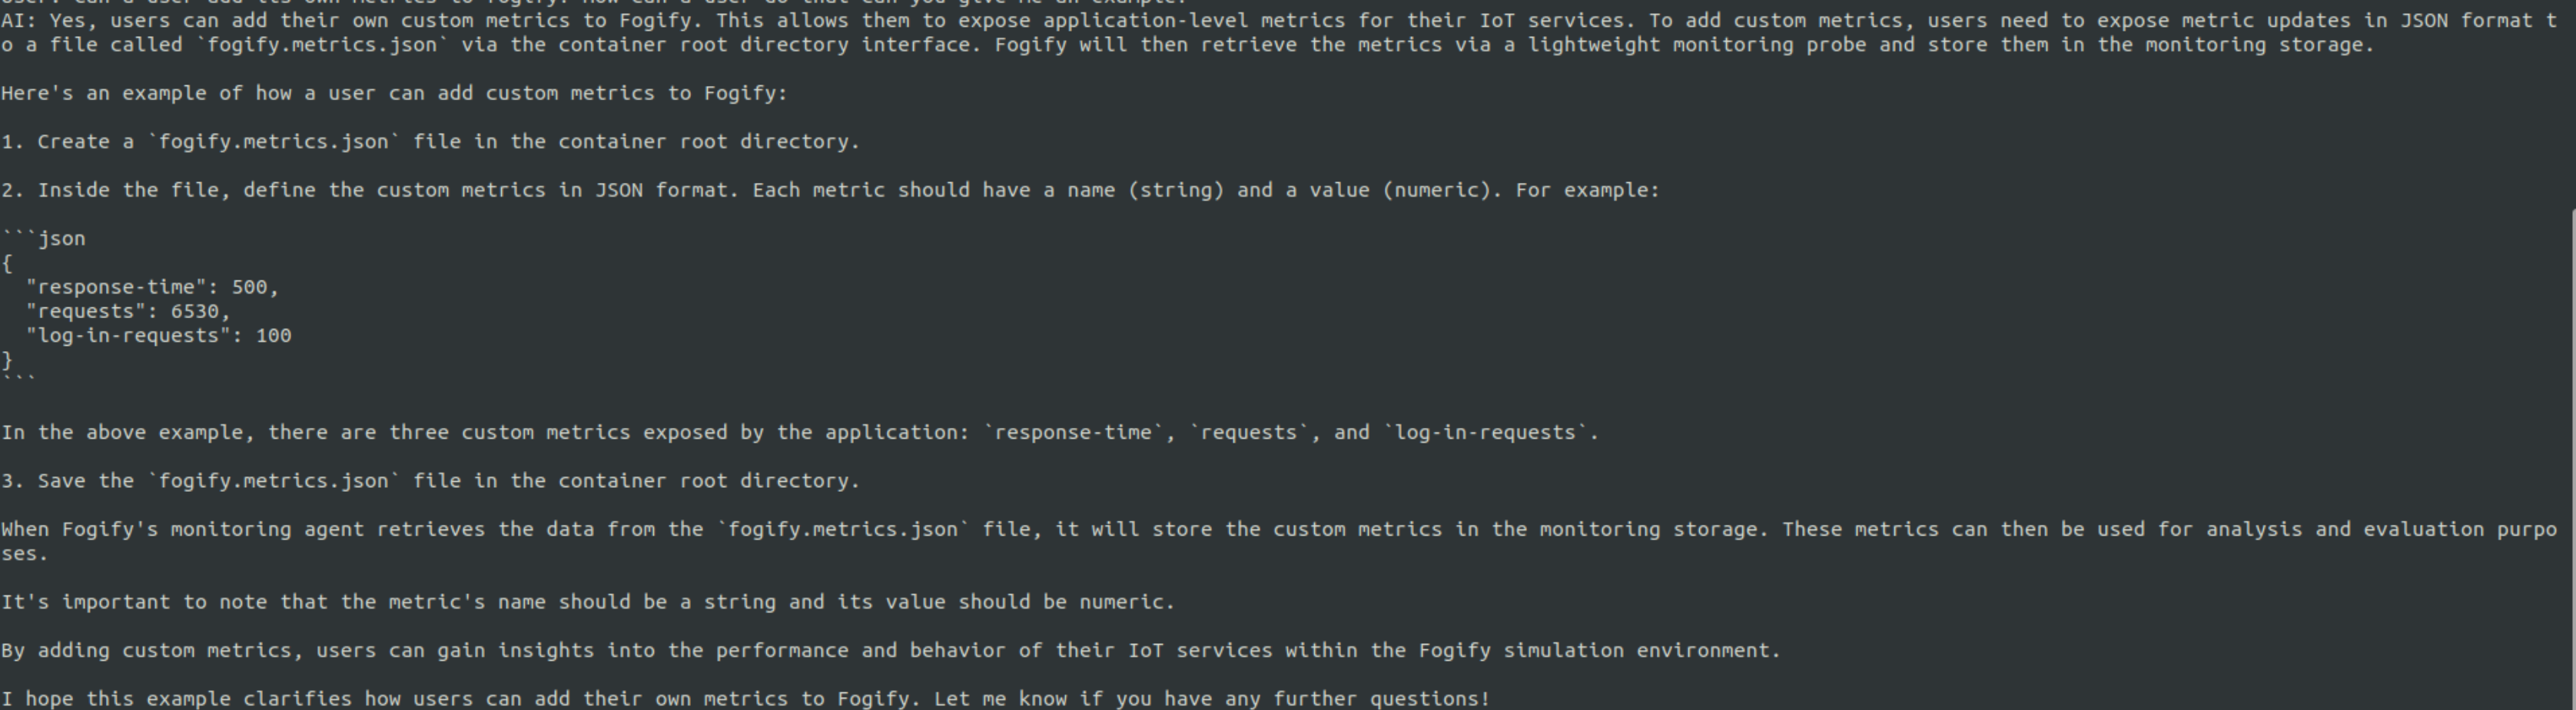
\includegraphics[width=8cm,height=4cm]{figures/q7.png}
              \caption[Methodology pipline]{Answer for question 7}
              \label{img:q7}
          \end{figure}
    \item How can someone interact with the emulated testbed?
          \begin{itemize}
              \item
          \end{itemize}
          \begin{figure}[h!]
              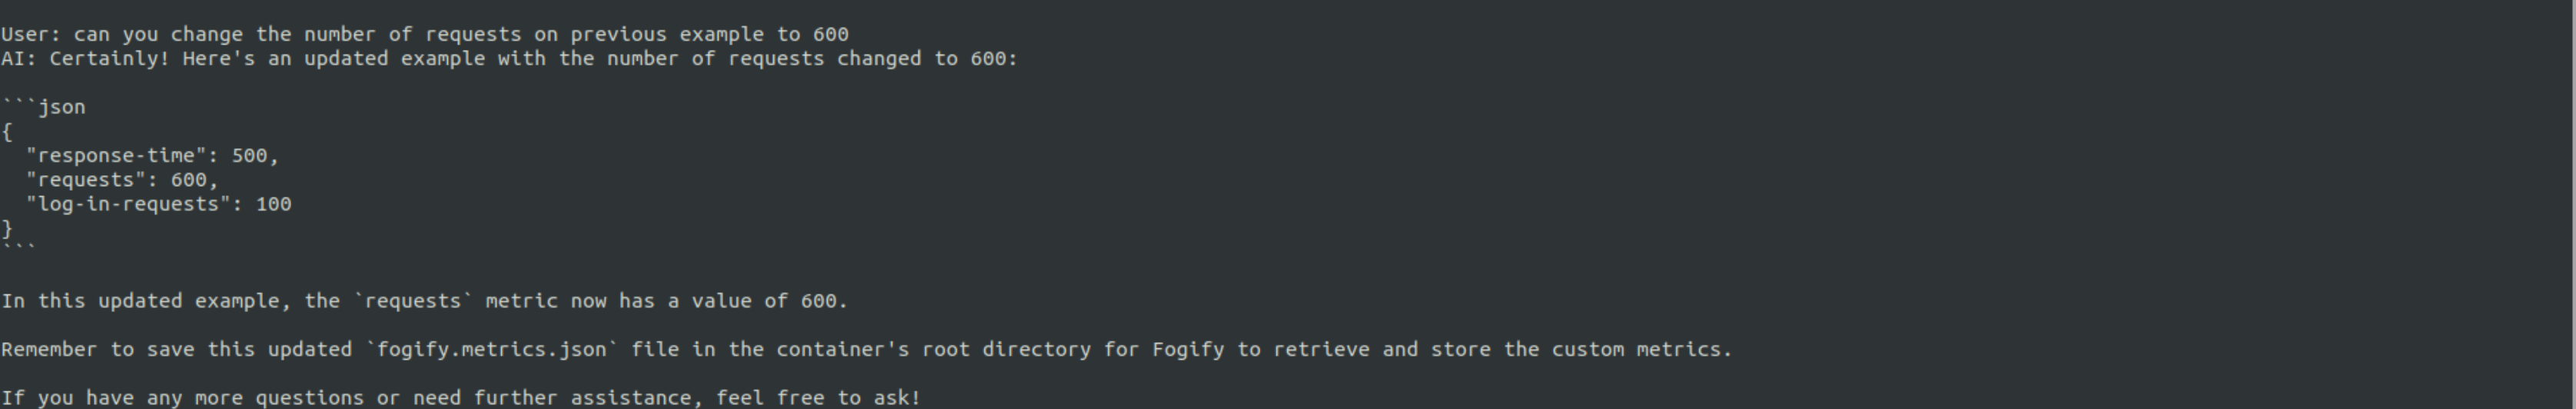
\includegraphics[width=8cm,height=4cm]{figures/q8.png}
              \caption[Methodology pipline]{Answer for question 8}
              \label{img:q8}
          \end{figure}
    \item Can you give me an example in python code on how i can use the fogify
          SDK library to interact with the Fogify emulation tool?
          \begin{itemize}
              \item
          \end{itemize}
          \begin{figure}[h!]
              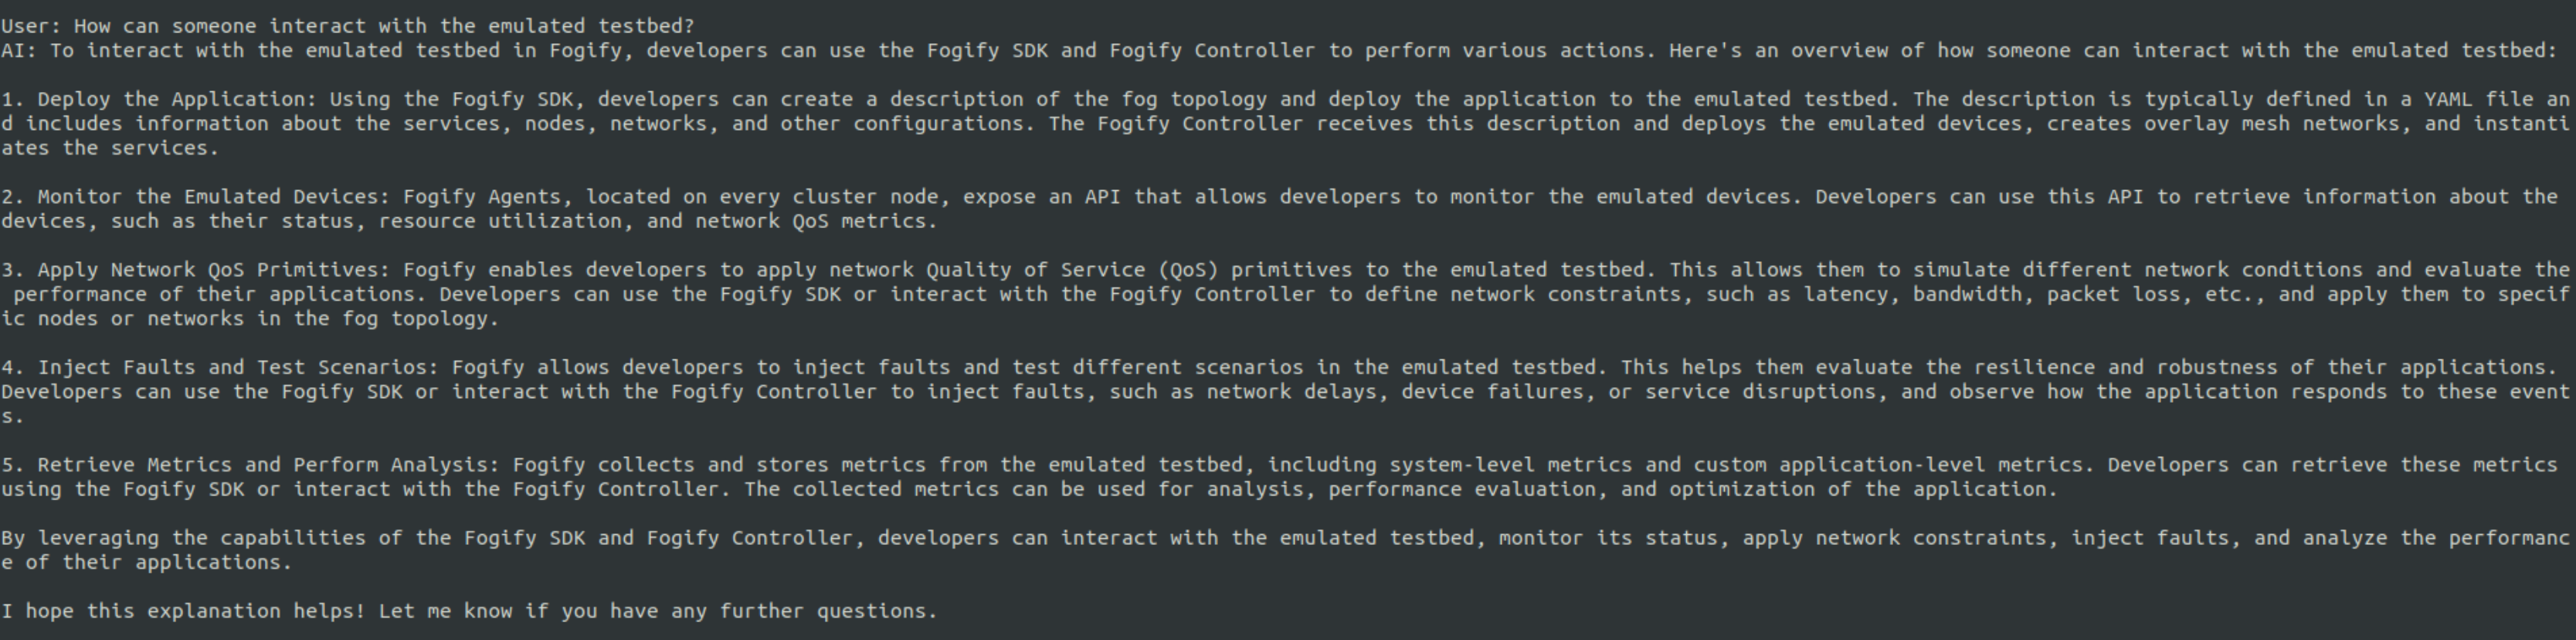
\includegraphics[width=8cm,height=4cm]{figures/q9.png}
              \caption[Methodology pipline]{Answer for question 9}
              \label{img:q9}
          \end{figure}
\end{enumerate}
